\subsection{Cost of Capital}

Recall that the weight average cost of capital (WACC) is as follows:
\begin{equation}
\text{WACC} = w_e r_e + w_p r_r + w_d r_d (1-t) \nonumber 
\end{equation}
where $r_e$ is cost of equity, $r_p$ cost of preferred equity, $r_d$ cost of debt, and $w_e, w_r, w_d$ cost of weights. Consider the after-tax cost of debt if interest expense is tax-deductible, using the marginal tax rate.

\subsubsection{Cost of Capital Factors}

\begin{remark} Top-down factors that impact cost of capital are as follows:
\begin{enumerate}[label=\roman*.]
\setlength{\itemsep}{0pt}
\item \hlt{Capital Availability}: if economy has greater availability of capital, the cost will be lower. Developed economies with established, liquid capital markets, more stable currencies, better protection and law will have lower cost of capital. In some less-developed markets with lack of corporate debt markets, companies rely on other means for funding, such as bank loans or shadow banking system.
\item \hlt{Market Conditions}: lower expected inflation lead to lower nominal risk-free rates. Risk premiums on debt and equity decrease during economic expansions, and increase during economic contractions. Transparent and predictable monetary policies lead to lower risk premiums and interest rates. Higher currency volatility leads to higher risk premiums for risk-averse investors.
\item \hlt{Legal and Regulatory Considerations, Country Risk}: countries that follow common law-based legal systems have stronger legal systems, hence lower risk premiums compared to that of civil law-based legal systems.
\item \hlt{Tax Jurisdiction}: the higher the marginal tax rate, the greater the tax benefit of using debt.
\end{enumerate}
\end{remark}

\begin{remark} Bottom-up factors that impact cost of capital are as follows:
\begin{enumerate}[label=\roman*.]
\setlength{\itemsep}{0pt}
\item \hlt{Business or Operating Risk}: business with stable revenues, earnings and cash flows are less risky. Companies with higher customer concentration risk require more risk premium. Companies with higher leverage has higher volatility of earnings and cash flows require higher risk premiums. Companies with poor corporate governance, higher ESG-risk exposures will require higher risk premiums.
\item \hlt{Asset Nature and Liquidity}: companies with higher proportion of tangible, fungible assets have higher recovery rate, hence lower risk premium. Specialised assets and intangibles do not have a ready liquid market, hence have lower recovery rate. Assets designated as collateral reduce cost of secured debt, but increase cost of other subordinated unsecured debt as their claim becomes superior.
\item \hlt{Financial Strength and Profitability}: companies with higher profitability, higher ability to generate cash, lower leverage, have lower probability of default, hence a lower risk premium. 
\item \hlt{Security Features}: embedded call options increases current cost of borrowing for issuer, and allows company to refinance the debt at a favourable rate should if interest rates decline. Converse is true for put option. Cumulative preferred stock accumulates missed dividends when company is unprofitable, hence has lower risk premium. Common equity with inferior rights have higher costs than that of superior rights.
\end{enumerate}
\end{remark}

\begin{flushleft}
\begin{tabularx}{\textwidth}{X|p{5em}|p{5em}}
\hline
\rowcolor{gray!30}
Revenues, Earnings, and Cash Flow Volatility & Lower & Higher \\
\hline
Higher stability of revenues, earnings, and cash flows & \checkmark & \\
Higher revenue concentration & & \checkmark \\
Higher earnings predictability & \checkmark & \\
Higher operating leverage & & \checkmark \\
Higher financial leverage & & \checkmark \\
Higher ESG risks & & \checkmark \\
\hline
\rowcolor{gray!30}
Asset Nature and Liquidity & Lower & Higher \\
\hline
Higher proportion of fungible, tangible assets & \checkmark & \\
Higher proportion of liquid assets & \checkmark & \\
\hline
\rowcolor{gray!30}
Financial Strength, Profitability, and Financial Leverage & Lower & Higher \\
\hline
Higher profitability & \checkmark & \\
Higher cash flow generation & \checkmark & \\
Higher interest coverage ratio, liquidity & \checkmark & \\
Higher leverage ratio & & \checkmark \\
\hline
\rowcolor{gray!30}
Security Features & Lower & Higher \\
\hline
Debt: call features & & \checkmark \\
Debt: put features & \checkmark & \\
Debt: conversion feature & \checkmark & \\
Preferred Equity: cumulative feature & \checkmark & \\
Common Equity: inferior cash flow or voting rights & & \checkmark \\
\hline
\end{tabularx}
\end{flushleft}

\subsubsection{Cost of Debt Estimation}

\begin{method} \hlt{Traded Debt}\\
If corporate debt is publicly traded, the yield to maturity (YTM) for longest maturity straight debt (debt with no embedded options) is the best estimate of cost of debt. If there exists shorter-term bonds that are more liquid than longest dated bond, YTM for this may be used instead.	
\end{method}

\begin{method} \hlt{Non-Traded Debt}\\
For private companies, or public companies with non-traded or illiquid debt securities.\\
If credit rating exists, estimate YTM with matrix pricing by considering bonds of other companies with same or similar maturities and credit ratings. If credit rating does not exist, use interest coverage ratio or financial leverage ratio to deduce credit rating.\\
Alternatively, credit spread of specific credit rating and maturity may be applied to benchmark rates.\\
Note, a company may have different ratings depending on debt collateral, seniority, convertibility, and other features. Hence, issuer rating may differ from issuer's individual series of debt.
\end{method}

\begin{method} \hlt{Bank Debt}\\
Determine interest on new bank debt financing for company to estimate cost of bank debt; if new bank debt is recent, then this may be good estimate of cost of debt if interest rate reflects current market conditions, and company risk profile has not changed materially since issuance.
\end{method}

\begin{method} \hlt{Leases}\\
A finance or capital lease is an example of amortised loan, and can be used to estimate cost of borrowing. The rate implicit in the least (RIIL) is the implied cost of capital, which is IRR from:
\begin{equation}
\text{PV of lease payments} + \text{PV of residual value} = \text{Fair value of leased asset} + \text{Lessor's direct initial cost} \nonumber
\end{equation}
If present value of residual value and lessor's direct initial costs are unknown, the incremental borrowing rate (IBR) (rate on new secured loan over same term) may be used.
\end{method}

\begin{method} \hlt{International Considerations for Cost of Debt Estimation}\\
For foreign market, country risk premium is added to debt's yield.\\
A country risk rating (CRR) may be used, which reflects risk related to economic conditions, political risk, exchange rate risk, securities market development and regulation. Country may be assigned a rating relative to benchmark country, which excess of the median interest rate relative to benchmark is the CRR.
\end{method}

\subsubsection{Cost of Equity Estimation}

\begin{method} \hlt{Equity Risk Premium (ERP) Historical Estimates}\\
Approach used when reliable long-term equity return data is available. Typically calculated as mean value of difference between broad-based equity index return and a government debt return (as proxy for risk-free rate).\\
Returns are assumed to be stationary, markets relatively efficient. Decisions to make includes:
\begin{enumerate}[label=\roman*.]
\setlength{\itemsep}{0pt}
\item Equity Index Selection: select an index that accurately represents typical returns earned by equity investors. Broad-based, market-value-weighted indexes typically chosen.
\item Time Period: longer time period that covers multiple business cycles and variety of market conditions should be covered. Older data may not reflect current market conditions,
\item Selection of Mean Type: arithmetic mean is easy to calculate, but is sensitive to extreme values, and overestimated the expected terminal value of wealth. Geometric mean gives outliers less weight, and estimates the expected terminal value of wealth more accurately, hence is more preferred.
\item Selection of Risk-Free Rate Proxy: as duration of equity is long-term (infinite), long-term government bond rates is preferred as proxies for risk-free rate\\
\begin{tabularx}{\textwidth}{p{12.5em}|X|X}
\hline
\rowcolor{gray!30}
Risk-Free Proxy & Advantages & Disadvantages \\
\hline
Short-Term Govt Bill Rate & Exact estimate of risk-free rate, assuming no default & does not closely match duration of infinite-life equity security \\
\hline
Long-Term Govt Bond YTM & YTM more closely match duration of infinite-life equity security & YTM not completely risk-free (unknown coupon reinvestment rates) \\
\hline
\end{tabularx}
\end{enumerate}
\end{method}

\begin{remark} \hlt{Limitations of Historical Approach for Computing ERP}
\begin{enumerate}[label=\roman*.]
\setlength{\itemsep}{0pt}
\item ERPs are countercyclical; low during economic expansion, high during contractions. Estimates based on long time series of historical data is not representative of future ERP.
\item Survivorship bias inflate historical estimates of ERP. Bias is in equity market data when poorly performing or defunct companies are removed from index membership.
\end{enumerate}
\end{remark}

\begin{method} \hlt{Equity Risk Premium (ERP) Forward-Looking Approach}\\
Approach uses current information and expectations on economic and financial variables. Do not rely on assumption of stationarity, and less affected by survivorship bias.
\end{method}

\begin{method} \hlt{Forward-Looking Approach: Survey-Based Estimates}\\
Uses consensus of opinions from experts. Surveys tend to higher ERPs for developing markets relative to developed markets. Biased toward recent market returns.
\end{method}

\begin{method} \hlt{Forward-Looking Approach: Dividend Discount Model Estimates}\\
Simplified model uses expected constant earnings growth rate (Gordon Growth Model), and solving for required return on equity yields
\begin{equation}
r_e = \frac{D_1}{V_0} + g \nonumber
\end{equation}
where $V_0$ is present value of future expected dividends, $\frac{D_1}{V_0}$ is expected dividend yield, $g$ is expected earnings growth rate. Broad-based equity indexes have associated dividend yield, and year-ahead dividend $D_1$ may be fairly predictable. Expected earnings growth rate $g$ may be inferred based on analyst expectations, which can be top-down or bottom-up generated forecasts.\\
Subtracting current risk-free rate from expected market equity return yields forward-looking ERP:
\begin{equation}
\text{ERP} = E\left[\frac{D_1}{V_0}\right] + E[g] - r_f \nonumber 
\end{equation}
Constant growth model assumes constant growth rate in earnings and dividends; else an adjustment on anticipated P/E multiple expansion or contraction needs to be done. P/E increase may be due to increase in earnings growth rate or decrease in risk (vice versa). \\
Aggregate amount spent on buybacks by index constituent companies may be included in dividend yield to reflect total payout; consider degree to which buyback alter growth rates in earnings and dividends.\\
For rapidly growing economies, a three stage growth model (fast, transition, mature) may be used. 
\begin{equation}
\text{Equity Index Price} = PV_{\text{Fast}} + PV_{\text{Transition}} + PV_{\text{Mature}} \nonumber
\end{equation}
The $IRR$ from this is then the required rate of return. Subtract current risk-free rate to get ERP.
\end{method}

\begin{method} \hlt{Forward-Looking Approach: Macroeconomic Model}\\
Grinold-Kroner model is used, which decomposes ERP as follows:
\begin{align}
\text{ERP} &= [\text{Dividend Yield} + \text{Capital Gains Yield}] - E[r_f] \nonumber \\
&= [\text{Dividend Yield} + \text{Expected Repricing} + \text{Earnings Growth per Share}] - E[r_f] \nonumber \\
&= \left[DY + \Delta (P/E) + i + g - \Delta S \right] - E[r_f] \nonumber
\end{align}
\begin{tabularx}{\textwidth}{p{14em}|p{4em}|X}
\hline
\rowcolor{gray!30}
Factor & Symbol & Common Proxy \\
\hline
Expected income component & DY & Broad-based market index dividend yield \\
\hline
Expected growth rate in P/E & $\Delta (P/E)$ & Adjust for market over or under valuation (commonly $0$) \\	
\hline
Expected inflation & $i$ & (nominal yield $-$ real yield) for similar maturity security \\
\hline
Expected growth in real EPS & $g$ & Real GDP growth \\
\hline
Expected $\Delta$\% in shares outstd & $\Delta S$ & Depends on market and time period \\
\hline
\end{tabularx}\\

Common approach to estimate expected inflation is to compare nominal yield on US Treasury bond to yield on equivalent inflation-protected Treasury security (TIPS):
\begin{equation}
i = \frac{1 + \text{YTM}_{\text{Treasury Bond}}}{1 + \text{YTM}_{\text{TIPS}}} - 1 \approx \text{YTM}_{\text{Treasury Bond}} - \text{YTM}_{\text{TIPS}} \nonumber
\end{equation}
\end{method}

\begin{remark} \hlt{Limitations of Forward-Looking Approach for Computing ERP}\\
\begin{tabularx}{\textwidth}{p{5em}|X}
\hline
\rowcolor{gray!30}
Factor & Symbol \\
\hline
Surveys & Subject to sampling and response biases, behavioural biases (recency bias, confirmation bias) \\
\hline
DDM & Assumes constant P/E. Adjustment on P/E to reflect multiple expansion or contraction \\
\hline
Macroecon & Models may have modelling errors or behavioural biases in forecasting \\
\hline
\end{tabularx}
\end{remark}

\begin{method} \hlt{ERP Estimation: Dividend Discount Model}\\
For individual company, cost of equity is dividend yield plus capital gains yield.
\begin{equation}
r_e = \frac{D_1}{P_0} + g \nonumber
\end{equation}
A multi-year forecast may be built, in this case we may solve for $r_e$ in following equation:
\begin{equation}
P_0 = \left[ \sum\limits_{t=1}^n \frac{D_t}{(1+r_e)^t} \right] + \frac{P_n}{(1+r_e)^n} \nonumber
\end{equation}
\end{method}

\begin{method} \hlt{ERP Estimation: Risk-Based Models}\\
Let $r_e$ be sum of compensation for time value of money and for bearing risk.
\begin{enumerate}[label=\roman*.]
\setlength{\itemsep}{0pt}
\item Capital Asset Pricing Model (CAPM): single factor model,
\begin{equation}
r_e = r_f + \hat{\beta}(\text{ERP}) \nonumber
\end{equation}
where $r_f$ is risk-free rate, $\hat{\beta}$ is company beta.\\
This may be estimated with market model, which replaces expected returns on company and market with actual historical returns. Let $r_{i,t}$ be equity excess returns, $r_{f,t}$ be risk-free rate, $r_{m,t}$ be excess returns of an equity market index. Then
\begin{equation}
(r_{i,t} - r_{f,t}) = b_0 + b_1 (r_{m,t} - r_{f,t}) + \epsilon_t \nonumber
\end{equation}
For private companies, beta of a comparable publicly traded company may be used by after adjusting for leverage differences.
\item Fama-French Models: multi-factor model that adds two additional factors to CAPM:
\begin{equation}
r_e = r_f + \beta_1 \text{ERP} + \beta_2 \text{SMB} + \beta_3 \text{HML} \nonumber
\end{equation}
where SMB is size premium, HML is value premium (measured by book-to-market ratio).\\
The five factor model adds profitability factor (robust vs weak profitability) (RMW) and investment factor (conservative vs aggressive investment) (CMA):
\begin{equation}
r_e = r_f + \beta_1 \text{ERP} + \beta_2 \text{SMB} + \beta_3 \text{HML} + \beta_4 \text{RMW} + \beta_5 \text{CMA} \nonumber
\end{equation}
\end{enumerate}
\end{method}

\begin{method} \hlt{ERP Estimation: Private Companies}\\
As there is no market price data, CAPM and Fama-French is not suitable to be directly applied.\\
Illiquidity, lack of transparency (no security filings and disclosures), and ownership structure with greater concentration of control, increases investment risk.\\
Specific-company risk premium (SCRP) reflects factors such as geographic risk, key-person risk, and other firm-specific factors that may not be easy to diversity away.\\

\begin{tabularx}{\textwidth}{X|X}
\hline
\rowcolor{gray!30}
Qualitative Factors & Quantitative Factors \\
\hline
\xxx The industry in which the business operates
\xxx Competitive position within the industry
\xxx Management’s experience and expertise
\xxx Customer and supplier concentration
\xxx Geographic concentration of the business
\xxx Governance model of the company
\xxx Asset nature and type (tangible vs. intangible) 
&
\xxx Financial and operational leverage
\xxx Volatility in cash flows and earnings • Earnings predictability
\xxx Pricing power \\
\hline
\end{tabularx}
\\

Private company valuation also takes into account size premium (SP) and industry risk premium (IP).
\begin{enumerate}[label=\roman*.]
\setlength{\itemsep}{0pt}
\item Expanded CAPM: adds private company related risk premiums to CAPM
\begin{equation}
r_e = r_f + \beta_{\text{Peer}}(\text{ERP}) + \text{SP} + \text{IP} + \text{SCRP} \nonumber
\end{equation}
Estimate industry beta $\beta_{\text{Peer}}$ from peer group of publicly traded companies in same industry. Given estimate of $r_f$ and ERP, compute a CAPM estimate for $r_e$. Next, determine whether additional risk premium for company size and other company-specific risk factors are warranted, and add relevant size and company-specific risk premiums to arrive at final estimate of $r_e$.\\
SP is usually added to smaller private companies, inversely related to size of company. If lowest market-cap decile of public companies are used, then this is equal to return on average-systematic-risk micro-cap public equity issue. 
\item Build-Up Approach: starts with risk-free rate, adds relevant private company premiums.
\begin{equation}
r_e = r_f + (\text{ERP}) + \text{SP} + \text{SCRP} \nonumber
\end{equation}
ERP is not beta-adjusted, as this is the required return on equity for an average-systematic-risk large-cap public equity issue. 
\begin{figure}[H]
\centering
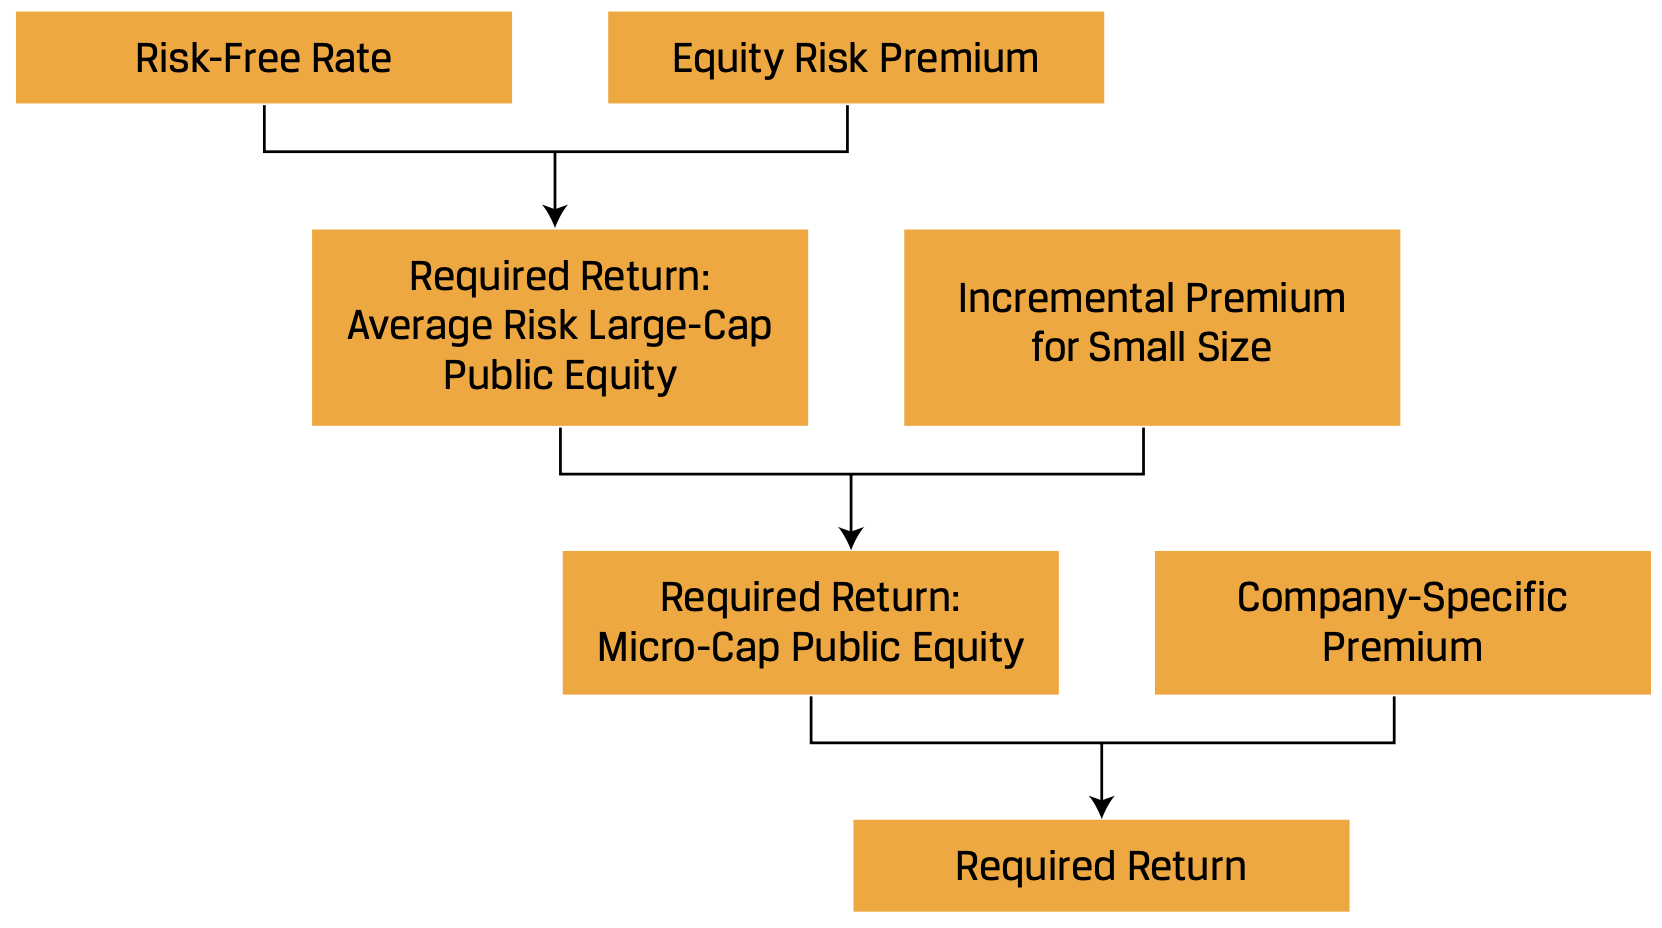
\includegraphics[scale=0.4]{/corpissuer/buildup}
\caption{Build-up approach for private companies.}
\end{figure}
Approach is suitable when set of comparable public companies are unavailable or incomparable.
\end{enumerate}
\end{method}

\begin{method} \hlt{ERP Estimation: International Considerations}\\
Risks for emerging market require additional premiums.
\begin{enumerate}[label=\roman*.]
\setlength{\itemsep}{0pt}
\item Country Spread Model: additional country risk premium (CRP) is to be added. The added risk could be due to economic conditions, risk of expropriation, political risk, or other risk.
\begin{equation}
\text{ERP}_{EM} = \text{ERP}_{DM} + (\lambda \times \text{CRP}) \nonumber
\end{equation}
where $\lambda$ is exposure of the company to the local company.\\
CRP is the premium associated with anticipated greater risk of market compared to benchmark developed market. Sovereign yield spread (yield difference in EM vs DM sovereign securities) may be used; but differences in legal and market environment complicates use of just yield spreads.\\
Aswath Damodaran suggests adjusting the sovereign yield spread by ratio of standard deviation of country's equity and bond markets as follows:
\begin{equation}
\text{CRP} = \text{Sovereign Yield Spread} \times \frac{\sigma_{\text{Equity}}}{\sigma_{\text{Bond}}} \nonumber
\end{equation}
\item Extended CAPM: for companies operating globally, two types of models may be used. If a company operations are global, GCAPM and ICAPM may both be used; however, if operations extend to EM, methodology is less clear (estimation using sovereign yield approach might be appropriate). \\
Global CAPM (GCAPM): global market index is used to estimate ERP. Beta coefficient usually quite low due to low correlation between EM and DM. A second factor representing the local market is sometimes included, but availability of reliable market index data is a concern in EM.\\
International CAPM (ICAPM): 2 factor model based on a global market index ($r_{gm}$) and a foreign currency-denominated, wealth-weighted market index ($r_c$):
\begin{equation}
E[r_e] = r_f + \beta_{G}[E[r_{gm}] - r_f] + \beta_{C}[E[r_c] - r_f] \nonumber
\end{equation}
The first factor of ICAPM captures company relationship with local economy relative to global economy (lower $\beta_{G}$ indicates lower integration of company with global economy). Second factor captures sensitivity of company CF to changes in its local currency value.\\
\end{enumerate}
\end{method}